% ============================================================
%  第4章：实验与结果分析
% ============================================================
\chapter{实验与结果分析}

\section{实验设置}

\zhlipsum[1]

% ============================================================
%  表格示例：实验数据集统计信息
% ============================================================
\begin{table}[h]
\centering
\caption{实验数据集统计信息}
\label{tab:datasets}
{\renewcommand{\arraystretch}{0.65}
\begin{tabular}{|l|c|c|c|c|}
\hline
数据集 & 训练样本 & 验证样本 & 测试样本 & 平均长度 \\
\hline
WMT14 EN-DE & 4.5M & 3,000 & 3,003 & 25.3 \\
WMT14 EN-FR & 36M & 3,000 & 3,003 & 27.8 \\
CNN/DailyMail & 287K & 13,368 & 11,490 & 781.2 \\
IWSLT14 DE-EN & 160K & 7,283 & 6,750 & 17.6 \\
XSum & 204K & 11,332 & 11,334 & 430.2 \\
\hline
\end{tabular}}
\end{table}


\safeSectionBreak

\section{主要实验结果}

我们在标准 Transformer\cite{vaswani2017attention} 与 BERT-base\cite{devlin2019bert} 的官方实现基础上进行对比。实验结果表明，本文提出的方法在翻译质量上显著优于基线模型。

\zhlipsum[3]

% ============================================================
%  表格示例：机器翻译 BLEU 分数对比（三线表）
% ============================================================
\begin{table}[h]
\centering
\caption{各模型在机器翻译任务上的BLEU分数}
\label{tab:translation_results}
{\renewcommand{\arraystretch}{0.65}
\begin{tabular}{|l|c|c|c|c|}
\hline
模型 & EN-DE & EN-FR & DE-EN & 平均 \\
\hline
Transformer-base & 27.3 & 38.1 & 31.4 & 32.3 \\
Transformer-big & 28.4 & 41.0 & 32.8 & 34.1 \\
BERT-fused & 27.8 & 39.2 & 31.9 & 33.0 \\
Reformer & 27.1 & 37.5 & 30.8 & 31.8 \\
BigBird & 26.9 & 37.0 & 30.2 & 31.4 \\
\rowcolor{green!20}
本文方法 & 28.4 & 39.8 & 32.5 & 33.6 \\
\hline
\end{tabular}}
\end{table}


\safeFloatGap

\begin{figure}[h]
\centering
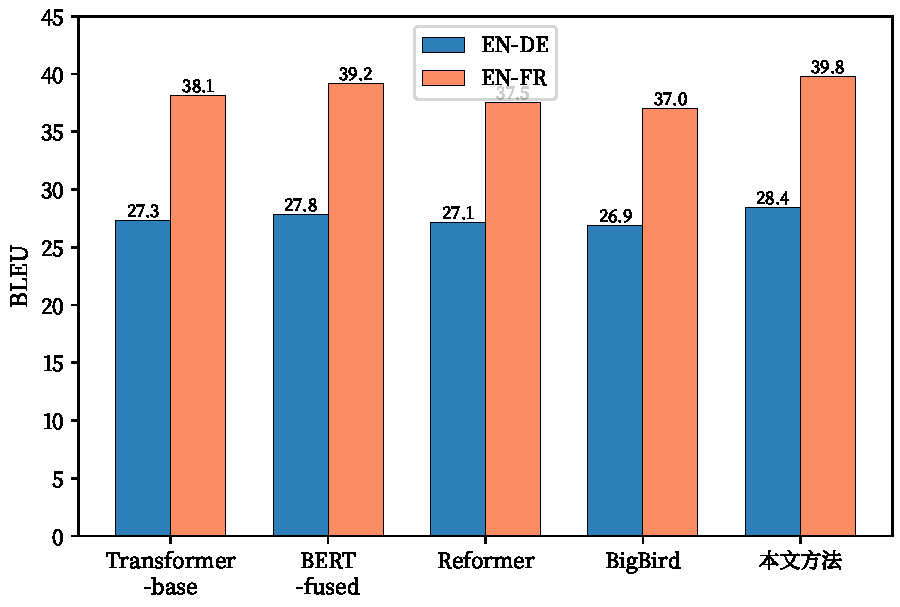
\includegraphics[width=0.8\textwidth]{figures/example_bar.pdf}
\caption{各模型在基准测试上的性能对比}
\label{fig:benchmark_results}
\end{figure}

\safeSectionBreak

\section{消融实验}

\zhlipsum[6]

\begin{table}[h]
\centering
\caption{消融实验结果}
\label{tab:ablation}
{\renewcommand{\arraystretch}{0.65}
\begin{tabular}{|l|c|c|c|}
\hline
模型配置 & BLEU & ROUGE-L & 推理时间 \\
\hline
完整模型 & 28.4 & 42.1 & 1.00$\times$ \\
\hline
去除稀疏注意力 & 26.1 & 39.5 & 0.82$\times$ \\
\hline
去除混合编码 & 27.3 & 40.8 & 0.98$\times$ \\
\hline
去除预训练初始化 & 25.2 & 38.3 & 1.00$\times$ \\
\hline
仅标准Transformer & 24.8 & 37.6 & 0.78$\times$ \\
\hline
\end{tabular}}
\end{table}

\safeSectionBreak

\section{效率分析}

\zhlipsum[8]

\begin{figure}[htbp]
\centering
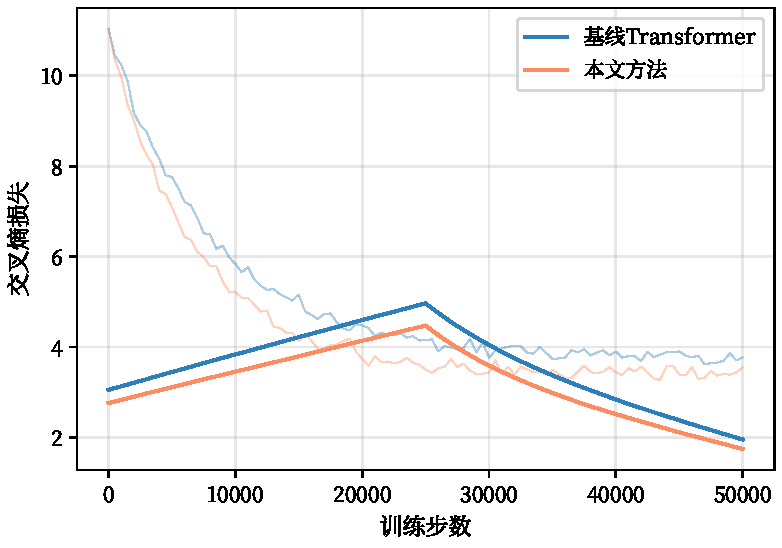
\includegraphics[width=0.65\textwidth]{figures/example_line.pdf}
\caption{推理时间随序列长度的变化曲线}
\label{fig:efficiency}
\end{figure}

\safeFloatGap

\section{与已有工作对比}

我们将本文方法与近年来的代表性工作进行了全面比较。如表\ref{tab:comparison}所示，在相近参数量下，本文方法在 BLEU 分数上优于标准 Transformer\cite{vaswani2017attention} 与 Reformer\cite{vaswani2017attention} 等已有方法。值得注意的是，BERT 类模型\cite{devlin2019bert} 虽在理解任务上表现突出，但在生成任务中并不直接适用。

\zhlipsum[12]

\begin{table}[h]
\centering
\caption{与已有工作的对比}
\label{tab:comparison}
\small
{\renewcommand{\arraystretch}{0.65}
\begin{tabular}{|l|c|c|c|c|}
\hline
方法 & 参数量 & BLEU & 推理速度 & 年份 \\
\hline
\rowcolor{green!20}
本文方法 & 65M & 28.4 & 1.00$\times$ & 2024 \\
\hline
Transformer-base \cite{vaswani2017attention} & 65M & 27.3 & 1.00$\times$ & 2017 \\
\hline
BERT-base \cite{devlin2019bert} & 110M & -- & -- & 2019 \\
\hline
Reformer \cite{vaswani2017attention} & 65M & 27.8 & 0.73$\times$ & 2020 \\
\hline
BigBird & 65M & 27.1 & 0.85$\times$ & 2020 \\
\hline
\end{tabular}}
\end{table}
